\documentclass[12pt]{article}
\usepackage{fullpage}
\usepackage{times}
\usepackage[normalem]{ulem}
\usepackage{fancyhdr,graphicx,amsmath,amssymb, mathtools, scrextend, titlesec, enumitem}
\usepackage[ruled,vlined]{algorithm2e} 
\usepackage{amsmath}
\include{pythonlisting}

\linespread{1.5}
\title{ECE335 Project 1}
\author{
  Wang, Jiashen\\
  \texttt{1001259568}
  \and
  Abukhadra, Sari\\
  \texttt{XXXXXXXXXX}
}
\date{\today}
\usepackage{graphicx}
\graphicspath{ {images/} }
\newcommand{\e}[1]{\times 10^{#1}}

\begin{document}
\vfill
\maketitle
\vfill

\newpage

\section{Zero Bias, Uniform Doping Profiles (10 Points)}

Using uniform doping profiles, verify the 1D and 2D impurity concentrations of the junction. Plot the 1D electrostatic potential across the junction to estimate the built-in potential and depletion region width. Compare the results with the theoretical values. [3+4+3]

\subsection{1D Electrostatic Potential Plot}
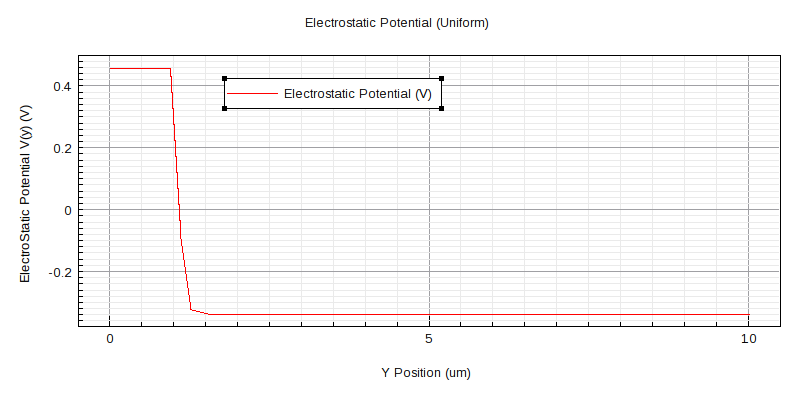
\includegraphics[width=\textwidth]{1a.png}
From the graph, the intrinsic potential is $0.46-(-0.336) = 0.796V$\\
The depletion width is $1.33 - 0.97 = 0.36um$
\subsection{Theoretical Calculation }
\begin{align*} 
\phi_{bi} &= \frac{kT}{q}\ln(\frac{N_d\cdot N_a}{N_i^2}) = 8.617\e{-5} \cdot 300\cdot \ln(\frac{2\e{18}\cdot8\e{15}}{(1.5\e{10})^2})=0.824V\\
W_{dep} &= (\frac{2\cdot \epsilon_{s}\cdot\phi_{bi}}{q}\cdot \frac{N_a+N_d}{N_a N_d})^{0.5}
= (\frac{2\cdot 11.7 \cdot 8.85\e{-14}\cdot 0.824}{1.609\e{-19}}\cdot \frac{8\e{15}+2\e{18}}{8\e{15} \cdot 2\e{18}})^{0.5}\\
&= 0.0000364 \text{cm} = 0.364 \text{um}
\end{align*}

\subsection{Comparision between the results }
The built in potential from the graph is slightly less than the theoretical calculation for the built in potential, perhaps because the junction is not perfectly divided in half as the p side is much larger. The theoretical built in potential assumes infinite length junction length. The depletion width is not very good at being measured on the graph, but it is slightly larger when its spread out on the p side.


\section{Reverse Bias, Uniform Doping Profiles (10 Points)}

Simulate the diode under reverse bias. Plot the reverse IV characteristics and extract the breakdown voltage. Compare your result with the following figure. What is the maximum electric field in the junction just before breakdown? [4+2+2+2]

\subsection{Plot and Extraction of Breakdown Voltage}
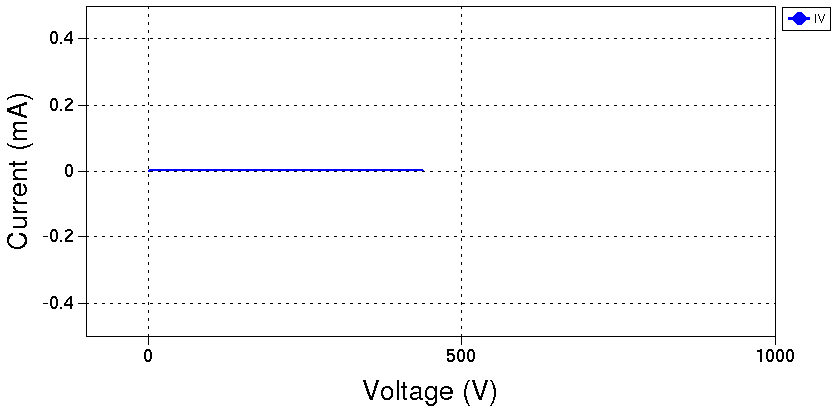
\includegraphics[width=\textwidth]{2a.png}
From the graph, the breakdown voltage is \textbf{~440V}

\subsection{Comparision with results and maximum electric field}

From the figure, with an impurity concentration of $8\e{15}  cm^{-1}$, the breakdown voltage is $700V$. The maximum electric field just before breakdown is 

\section{Forward Bias, Uniform Doping Profiles (8 Points)}

Plot the IV relation for this diode under a forward bias between 0 and 1 V. Identify and explain what happens as the forward bias is raised above 0.7V.
Hint: Examine the change in the IV relation with increasing voltage and determine the cause of this change. [4+4]

\subsection{IV Relation Plot and Explanation}
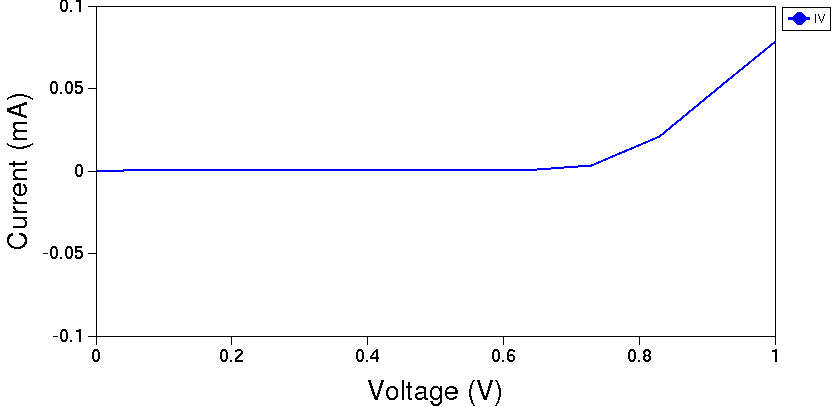
\includegraphics[width=\textwidth]{3a.png}

As the forward bias is raised above 0.7V, which is the threshold voltage is caused by the natural intrinsic voltage caused by the depletion region. Once it passes the depletion region the drift current starts going in one direction. 

\section {High Temperature, Uniform Doping Profiles (9 Points)}
The junction temperature is raised to 600°C. Simulate this junction up to a reverse bias of 10V and a forward bias of 1V. Plot and explain the IV characteristics. [4+5]

\subsection{Reverse Bias -10 to 0V}
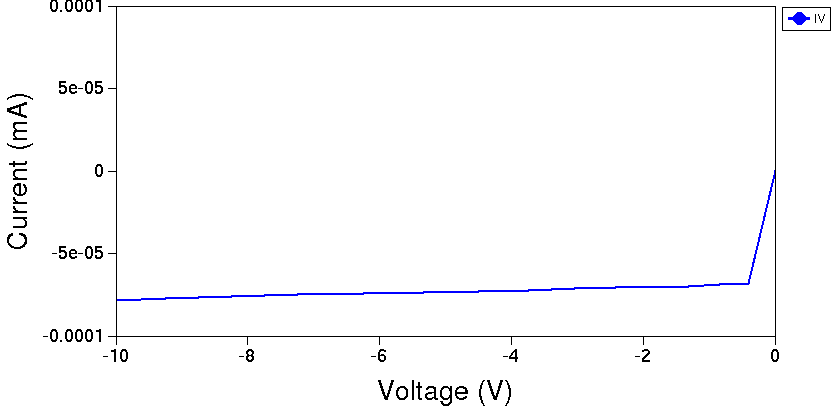
\includegraphics[width=\textwidth, height=200px]{4a.png}

\subsection{Forward Bias 0 to 1V}
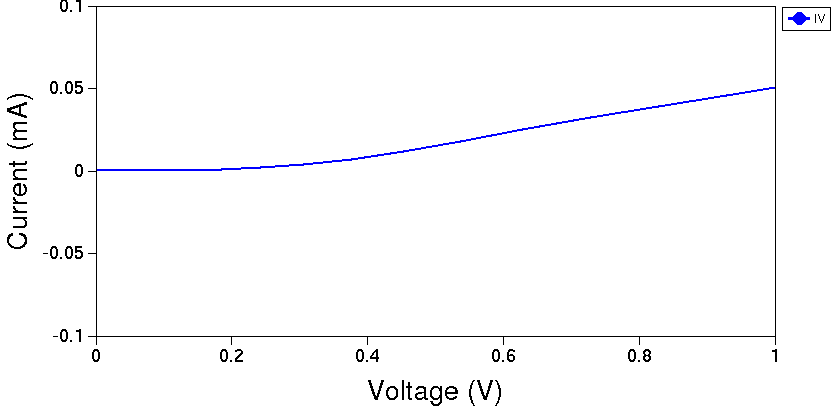
\includegraphics[width=\textwidth, height=200px]{4b.png}

\section{Gaussian n+ Doping Profile (18 Points)}
Using a Gaussian profile for the N+ region with peak concentration of 2×1018 cm−3, peak position of y = 0 μm, junction depth of 0.5 μm, the doping concentration at that depth is 1×1018 cm−3, and a Gauss factor of 0.8, verify the 1D and 2D doping concentration of the junction. Plot the 1D potential across the junction to estimate the built-in potential and depletion width at equilibrium. Compare the built-in potential with the theoretical value. Compare the built-in potential and depletion width to those of the uniformly doped diode (Part 1). Plot the IV relation of the diode between -2V and 1V and compare with that of the uniformly doped diode (Parts 2 and 3). Bonus: Estimate the minority carrier diffusion lengths Ln and Lp. [3+3+3+3+3+3 + (bonus 3)]



\end{document}